% Supplemental Material for Physical Review A Regular Article
% Compile locally with: latexmk -xelatex supplement.tex
\documentclass[11pt]{article}
\usepackage[a4paper,margin=2.1cm]{geometry}
\usepackage{fontspec}
\usepackage{unicode-math}
\IfFontExistsTF{TeX Gyre Termes}{
  \setmainfont{TeX Gyre Termes}
  \setmathfont{TeX Gyre Termes Math}
}{
  \setmainfont{Latin Modern Roman}
  \setmathfont{Latin Modern Math}
}
\usepackage{amsmath,booktabs,array,longtable,threeparttable}
\usepackage{graphicx}
\usepackage[hidelinks]{hyperref}
\usepackage[nameinlink,noabbrev]{cleveref}
\usepackage[font=small,labelfont=bf]{caption}
\newcommand{\Wraw}{W_{\mathrm r}}
\newcommand{\dd}{\mathrm{d}}
\newcommand{\ii}{\mathrm{i}}
\newcommand{\ket}[1]{\lvert #1\rangle}
\newcommand{\bra}[1]{\langle #1\rvert}
\newcommand{\expect}[1]{\langle #1\rangle}
\graphicspath{{figures/}{../figures/}{}}

\title{Supplemental Material:\\ Boundary-Selective Readout and Dissipative Backaction of a Two-Level Probe in a Finite Floquet Ising Chain}
\author{Weiyu Ruan}
\date{}

\begin{document}
\maketitle

\section*{Scope}

This Supplemental Material supplies the full numerical contract and retained-window checks for the main-text response, then displays the coupling, damping, and finite-size slices used to interpret the local TLS signal. It also documents the common-preparation geometry and matched-drive controls, the fixed eight-drive transfer test, channel/time diagnostics, hashes, and reproduction commands. The complete immutable task records remain in the versioned repository. No supplemental figure adds a drive, system size, propagation, or fit beyond the committed numerical artifacts.

\section{Detailed numerical and analysis contract}
\label{sec:supp-protocol}

The primary response data are generated from the complete finite chain--TLS density operator, not from the projected edge--TLS equations. In all principal $N=6$ calculations, $J=h=1$, the TLS is explicitly exchanged with one chain contact and amplitude-damped during both drive steps, and propagation applies the exact action of each piecewise-constant Liouvillian exponential through sparse matrix-exponential action. The reported two, four, or eight samples per half step control the continuous-time Fourier quadrature and phasor resolution; they are not Trotter integration steps. The chain has no additional relaxation or dephasing channel in the reported model. The projected model enters only as an interpretation whose spatial, spectral, channel, and damping consequences are tested against those full-model trajectories.

\begin{table}[ht]
\centering
\caption{Detailed numerical and analysis conventions.}
\label{tab:supp-protocol}
\small
\begin{tabular}{>{\raggedright\arraybackslash}p{0.31\linewidth}>{\raggedright\arraybackslash}p{0.55\linewidth}}
\toprule
Item & Convention \\
\midrule
Physical preparation & $\left(\ket{\uparrow_z}\bra{\uparrow_z}\right)^{\otimes N}\otimes\ket{0_d}\bra{0_d}$ for every Gate A v3 full-model trajectory; no topology-dependent pair or mode selection. \\
Primary detector observable & Baseline-subtracted complex TLS transverse phasor at $\Omega/2$, reported versus $r=\omega_d/(\Omega/2)$. \\
Gate A v3 grid & Eleven frozen ratios $r=0.880,0.904,\ldots,1.120$; $\Wraw=\int\dd r\,|A_{\rm TLS}(r)|^2$ retains declared directional order. \\
Backaction observables & $A_{\rm edge}$ is the magnitude of the baseline-subtracted $\Omega/2$ phasor of $\expect{Z_0(t)}$; $M_{\pi,{\rm edge}}$ is the magnitude of the alternating stroboscopic mean; $P_{\rm em}=\gamma_1\overline{\expect{n_d}}$. \\
Resolved spectroscopy & A splitting is fitted only for internally resolved completed spectra; unresolved points are retained graphically but excluded from the linear fit. \\
Channel/time bridge & Exact N=4 channel pair is compared to an independently initialized late-time damped-cosine fit; N=6 records are residual-qualified targeted near-$-1$ diagnostics. \\
Phase display & Relative phase is omitted near vanishing amplitudes; no phase unwrap is assigned physical meaning in that regime. \\
Sensitivity & Temporal grids of 2, 4, and 8 samples per half step and discards of $8T$, $20T$, and $40T$ are deterministic checks, not replicate statistics. \\
\bottomrule
\end{tabular}
\end{table}

\subsection{Separation of numerical campaigns}

The datasets used for the central claim and for the mechanism discussion were produced under different analysis contracts and are not pooled. The common-product matched controls and geometry comparisons provide the primary finite-system evidence. Denser legacy scans are retained only where they resolve coupling, damping, or projected-model behavior.

\begin{table}[ht]
\centering
\caption{Preparation, grid, and evidentiary role of the completed numerical campaigns. Internal protocol names are included only for repository traceability.}
\label{tab:supp-campaigns}
\small
\begin{tabular}{>{\raggedright\arraybackslash}p{0.22\linewidth}>{\raggedright\arraybackslash}p{0.29\linewidth}>{\raggedright\arraybackslash}p{0.39\linewidth}}
\toprule
Campaign & State, grid, and window & Observable and role \\
\midrule
Common-product matched controls (Gate A v3) & Explicit product state; 11 ratios $0.880$--$1.120$; pair-specific declared discard & $A_{\rm TLS}(r)$, $\Wraw$, and normalized distance; primary interpretive controls. \\
Common-product geometry controls (Gate A v3) & Same product state; six contacts or held-out OBC/PBC; same 11 ratios & Per-contact $\Wraw(x)$ and boundary-condition contrast; primary boundary evidence. \\
Dense spatial mechanism scan & Checkpoint scan; six contacts; 61 ratios $0.75$--$1.25$; discards $8T$, $20T$, $40T$ & $A_{\rm TLS}(x,r)$ and root-integrated-power profile; supplementary mechanism context only. \\
Coupling--frequency scan & Seven $g$ values; 61 ratios; discards $8T$, $20T$, $40T$ & Resolved TLS peak separation and its finite fitting window. \\
Damping scan & 31 rates at $g=0.08$, $r=1$; 80 periods; three discard windows & Edge/TLS phasors, emission proxy, and stroboscopic $\pi$ component versus $\gamma_1T$. \\
Channel diagnostics & Exact $N=4$ benchmark; targeted $N=6$ edge-seeded Ritz records & Exact $N=4$ channel/time comparison and residual-qualified near-$-1$ evidence at $N=6$. \\
\bottomrule
\end{tabular}
\end{table}

\subsection{Sampling and transient-window sensitivity}

The production-drive baseline uses four continuous-time samples per half step and discards the first $20T$. Relative to this baseline, two and eight samples per half step give normalized-shape distances $0.00106$ and $0.000311$ and raw-weight ratios $1.00187$ and $0.99911$. Changing only the discard to $8T$ and $40T$ gives distances $0.176876$ and $0.046216$ and raw-weight ratios $1.04122$ and $0.93229$, respectively. The intentionally early window therefore retains visible transient contamination, whereas the later window preserves the reported spectral shape within the predefined $D\le0.10$ tolerance. These are deterministic numerical checks, not confidence intervals.

\begin{figure}[ht]
\centering
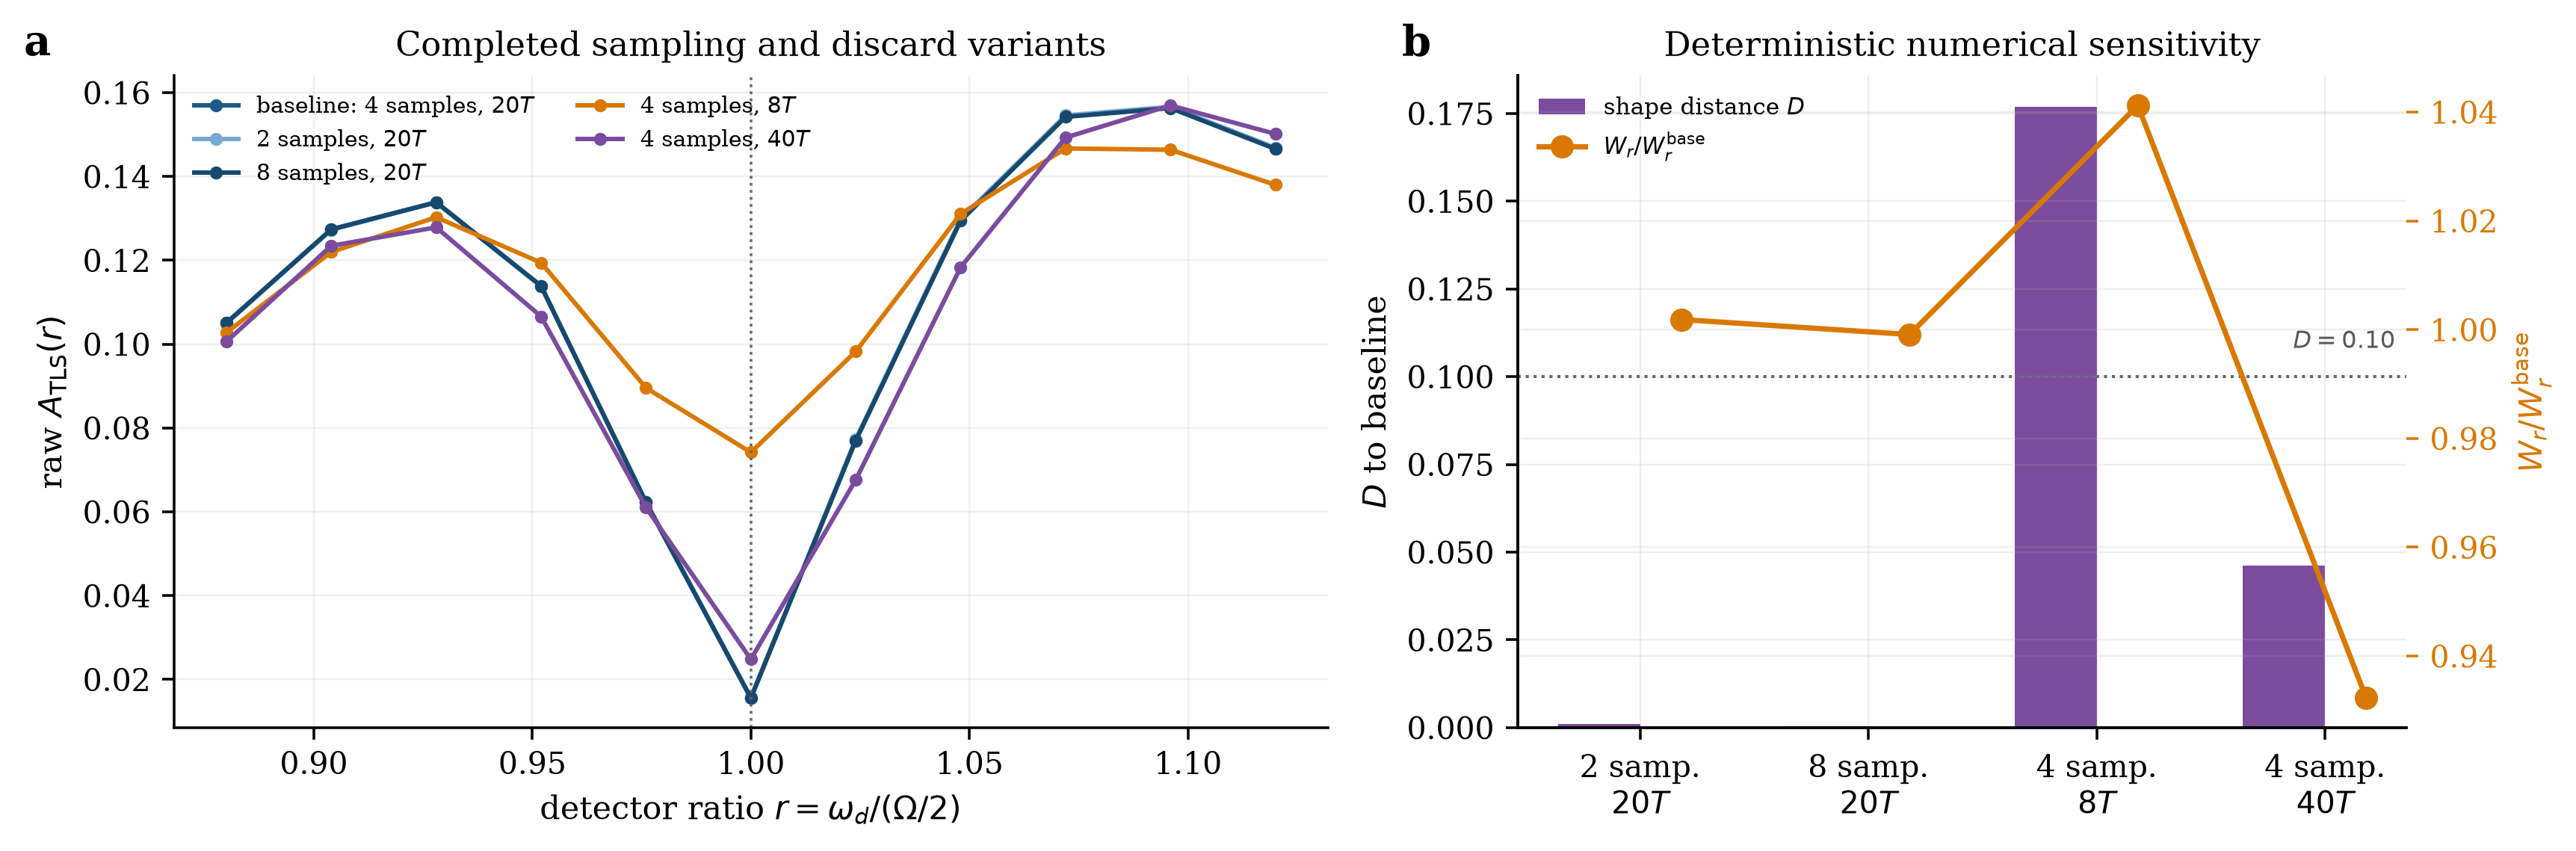
\includegraphics[width=\textwidth]{fig4_window_validation.png}
\caption{Sampling-density and transient-window sensitivity of the production response. Because propagation uses matrix-exponential action, the sampling variants test Fourier/quadrature resolution rather than time-integration error. The early $8T$ discard diagnoses transient sensitivity; the $40T$ window provides a later-time comparison.}
\label{fig:supp-window-validation}
\end{figure}

\section{Full response scans behind the projected edge--TLS theory}
\label{sec:supp-physics}

The reduced-model notation reserves $x$ for the physical TLS contact and $\ell\in\mathbb Z$ for the Floquet harmonic. With $B_{0\pi}(x,\ell)=T^{-1}\int_0^T\!\dd t\,e^{\ii\ell\Omega t}\bra{u_0(t)}\sigma_x^-\ket{u_\pi(t)}$, the interpretive sideband scale is $g_{x,\ell}=gB_{0\pi}(x,\ell)$ and the detuning is $\Delta_\ell=\omega_d-[(\epsilon_\pi-\epsilon_0)+\ell\Omega]$. The associated reduced equations use the fixed conjugation convention $c_d/c_e=-\ii g_{x,\ell}^*/(\gamma_2+\ii\Delta_\ell)$; hence its relative phase contains $-\arg g_{x,\ell}$, not $+\arg g_{x,\ell}$. In this projection, $\kappa_e$ denotes a phenomenological linewidth of the retained edge-sector amplitude and $f_e$ an effective source representing the physical preparation and discarded degrees of freedom. They are interpretive parameters, not fitted inputs used to generate any full-model curve. The following supplementary scans make explicit which numerical features are held fixed or varied in the main-text figures.

\subsection{Damping-window sensitivity}

The N=6 damping scan contains 31 logarithmically spaced bare TLS relaxation rates $0.005\le\gamma_1\le3$ at fixed $g=0.08$, nominal ratio one, and 80 periods. Every horizontal damping axis is reported as the dimensionless quantity $\gamma_1T$, with the fixed period $T=2.591813939212$. For a retained continuous-time record $z_0(t)=\expect{Z_0(t)}$, define
\begin{equation}
\widetilde A_{\rm edge}=\frac{2}{t_f-t_{\rm dis}}\int_{t_{\rm dis}}^{t_f}\!\dd t\,[z_0(t)-\overline{z_0}]e^{\ii\Omega t/2},\qquad A_{\rm edge}=|\widetilde A_{\rm edge}|.
\end{equation}
For the retained stroboscopic samples $z_{0,n}=\expect{Z_0(nT)}$, the code evaluates
\begin{equation}
M_{\pi,{\rm edge}}=\left|N_{\rm ret}^{-1}\sum_{n\in{\rm retained}}(-1)^n z_{0,n}\right|,
\qquad P_{\rm em}=\gamma_1\overline{\expect{n_d}}.
\end{equation}
The main-text crossover figure uses a 20-period discard. \Cref{fig:supp-damping-windows} shows the edge response, transverse TLS response, and edge $\pi$ component for 8-, 20-, and 40-period discards. The three windows preserve the qualitative suppression-and-recovery pattern; they are deterministic sensitivity checks rather than statistical replicates. In particular, the visibility-masked phase in the main text is not used as a surrogate for the amplitude data.

\begin{figure}[ht]
\centering
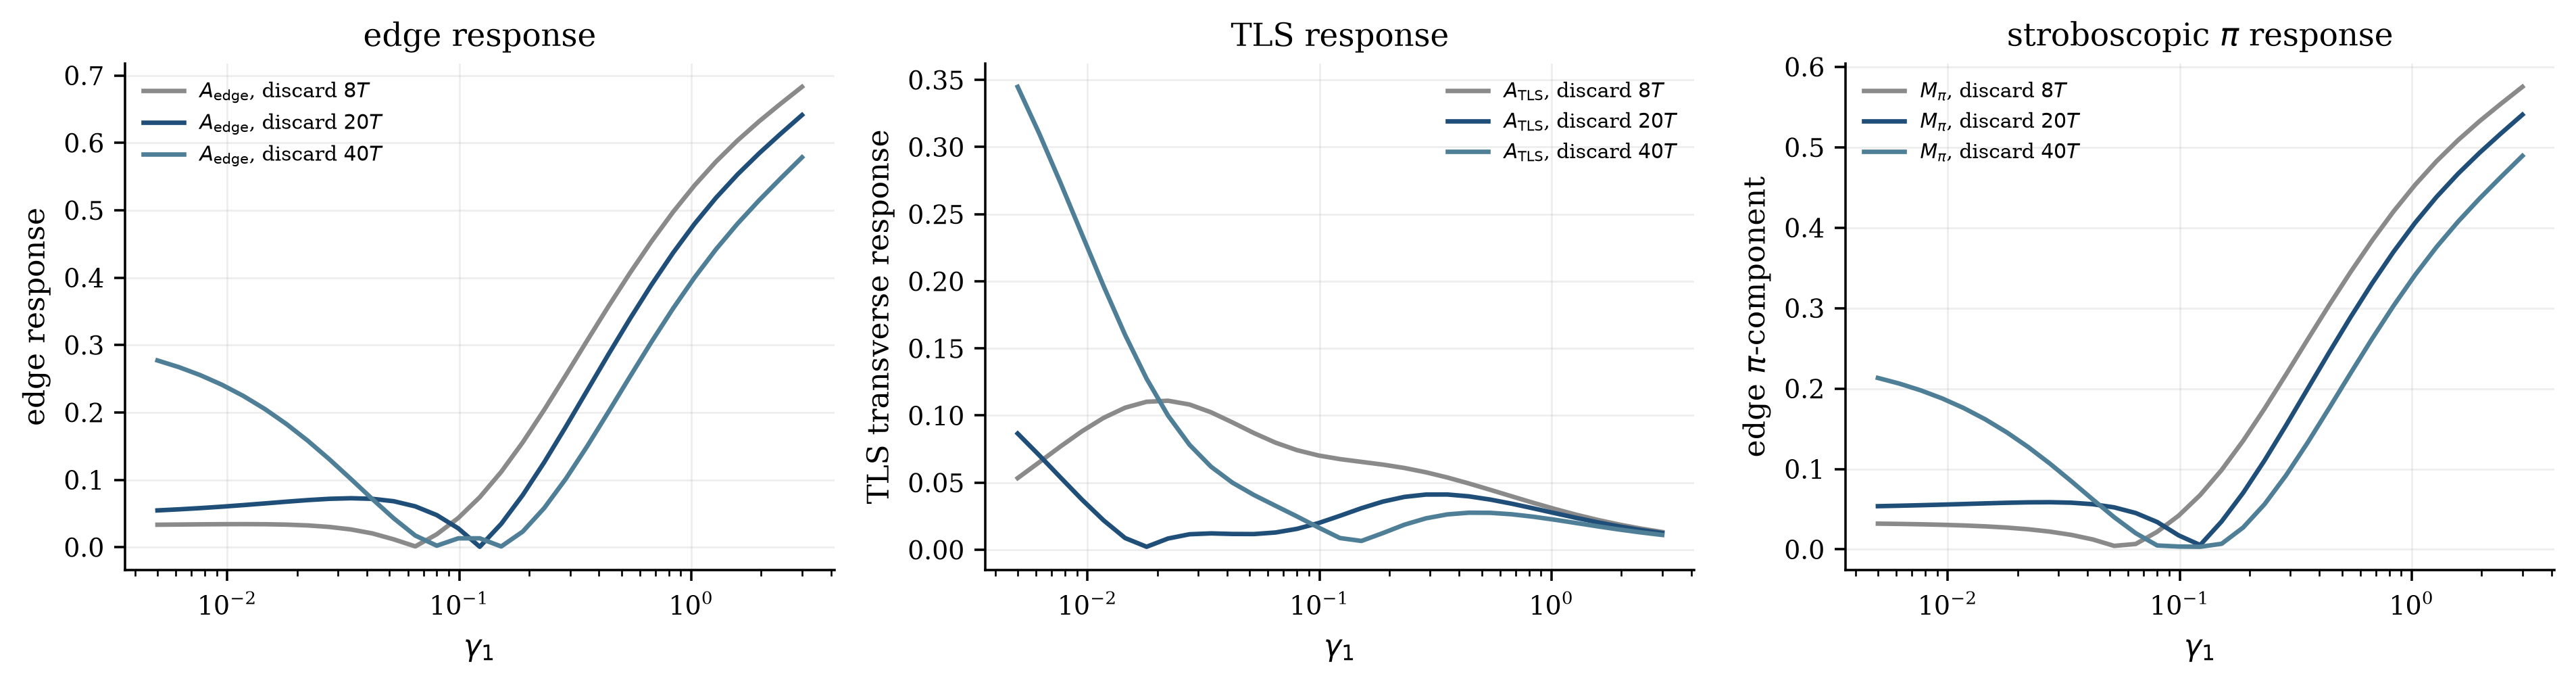
\includegraphics[width=\textwidth]{figS1_damping_window_sensitivity.png}
\caption{Three-window sensitivity of the N=6 damping sweep. Left to right: edge response, transverse TLS response, and stroboscopic edge $\pi$ component. The physical reading is a finite crossover, not a fitted phase transition.}
\label{fig:supp-damping-windows}
\end{figure}

\subsection{Finite-size readout slice}

The available open-chain size checkpoint compares $N=4$, $5$, and $6$ at a finite set of detector ratios. \Cref{fig:supp-size} reports the edge response, TLS transverse response, and emission proxy without extrapolating any quantity to infinite size. It is included to show the finite-size continuity of the measured readout variables, not to assert an asymptotic lifetime or localization law.

\begin{figure}[ht]
\centering
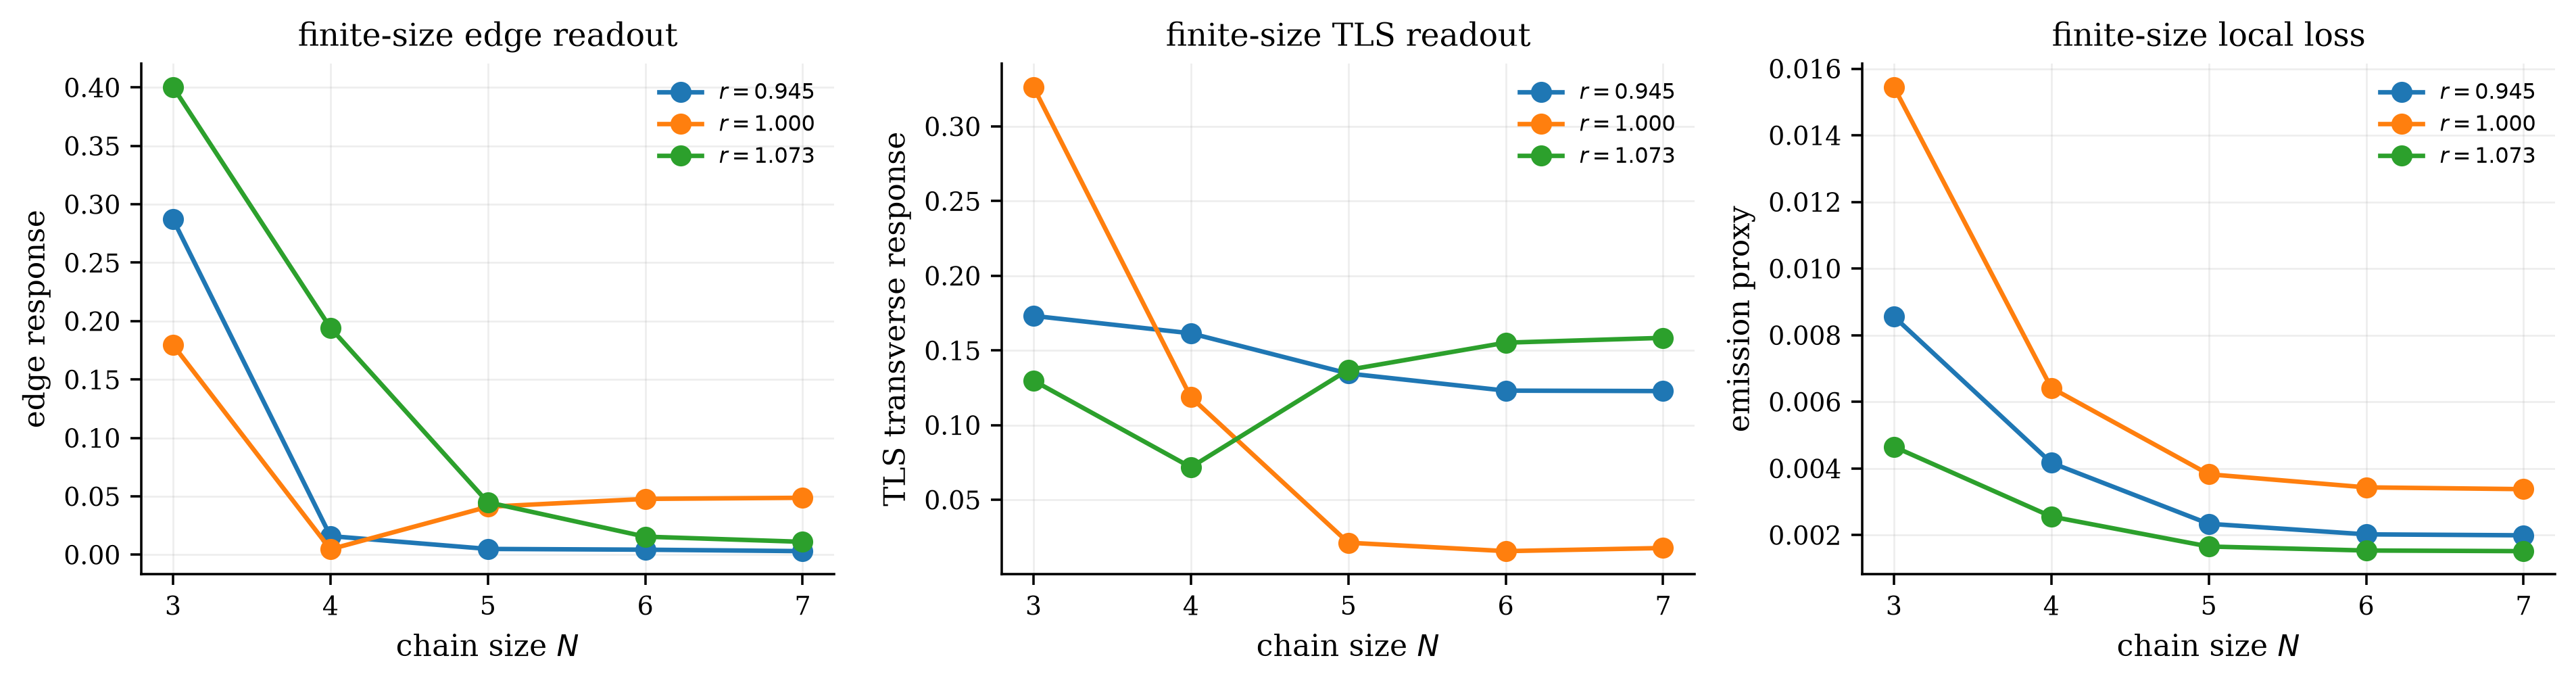
\includegraphics[width=\textwidth]{figS2_finite_size_readout.png}
\caption{Committed finite-size open-chain readout slice. Each curve is a completed response record at a fixed detector ratio. The panel provides finite-size context only; the work does not fit a thermodynamic scaling law from these three sizes.}
\label{fig:supp-size}
\end{figure}

\subsection{Complete coupling--frequency spectra}

The main text selects four representative spectra to make the resolved-doublet evolution legible. \Cref{fig:supp-coupling-spectra} gives all committed N=6 coupling--frequency curves. The splitting fit is restricted to the internally resolved points. The excluded/unresolved points are not dropped from the evidence record; they delimit the range in which the response can be summarized by a single resolved splitting.

\begin{figure}[ht]
\centering
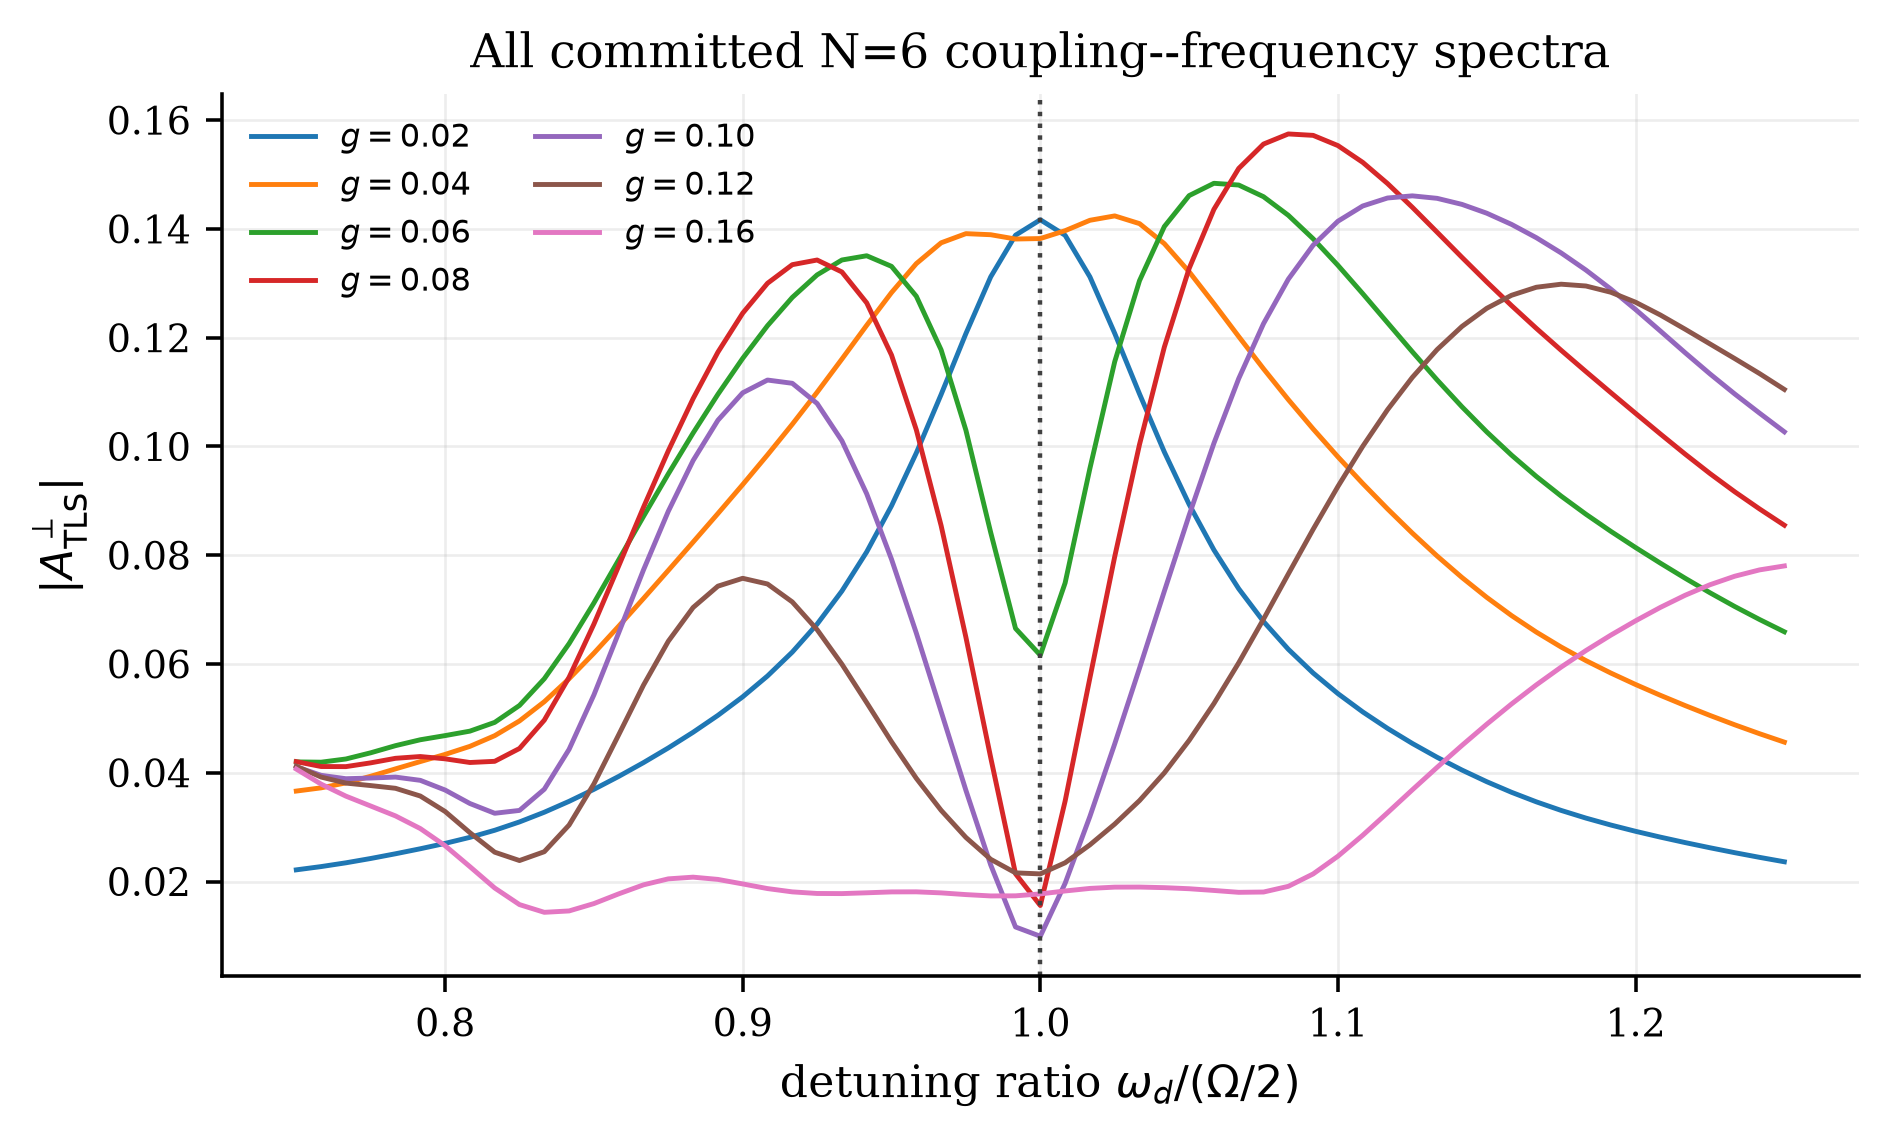
\includegraphics[width=0.72\textwidth]{figS3_all_coupling_frequency_spectra.png}
\caption{All committed N=6 coupling--frequency spectra used to identify the internally resolved hybridization range. The full set prevents the accepted linear scaling from being mistaken for a global all-coupling law.}
\label{fig:supp-coupling-spectra}
\end{figure}

\subsection{Fit diagnostics and detuning phase}

For the four accepted $20T$ scan settings, the full splitting is the mean of the extracted $8T$, $20T$, and $40T$ values; the vertical bars in the main-text figure are their sample standard deviations. An ordinary unweighted fit to bare $g/J$ gives
\begin{equation}
\frac{\Delta\omega}{J} = 3.452673\frac{g}{J}-0.0733333,
\qquad R^2=0.998248.
\end{equation}
The conditional ordinary-least-squares standard errors of the slope and intercept are $0.10227$ and $0.00948$, respectively, computed from the four point residuals with two residual degrees of freedom. They are descriptive fit errors, not experimental confidence intervals or a measure of systematic uncertainty in peak extraction. The fit constrained through the origin gives $\Delta\omega/J=2.685231(g/J)$ and $R^2=0.945884$. A fixed-contact re-expression using $|B_{0\pi}(0,0)|=0.2726796705$ rescales the horizontal axis without providing an independent matrix-element test. The nonzero intercept is therefore not interpreted as a nonzero splitting at $g=0$.

\begin{table}[ht]
\centering
\caption{Accepted coupling points and residuals of the free-intercept fit. All frequency quantities are in units of $J$; the window spread is deterministic.}
\label{tab:supp-coupling-residuals}
\begin{tabular}{rrrr}
\toprule
$g/J$ & Full splitting $\Delta\omega/J$ & Window s.d. & Fit residual \\
\midrule
0.06 & 0.137343 & 0.012414 & $+0.003516$ \\
0.08 & 0.198515 & 0.010949 & $-0.004365$ \\
0.10 & 0.270116 & 0.013492 & $-0.001818$ \\
0.12 & 0.343655 & 0.011486 & $+0.002667$ \\
\bottomrule
\end{tabular}
\end{table}

\Cref{fig:supp-detuning-phase} shows the separate production detuning sweep. The complex relative phase is displayed only where both edge and TLS phasor magnitudes exceed $0.02$; no phase is inferred at vanishing visibility.

\begin{figure}[ht]
\centering
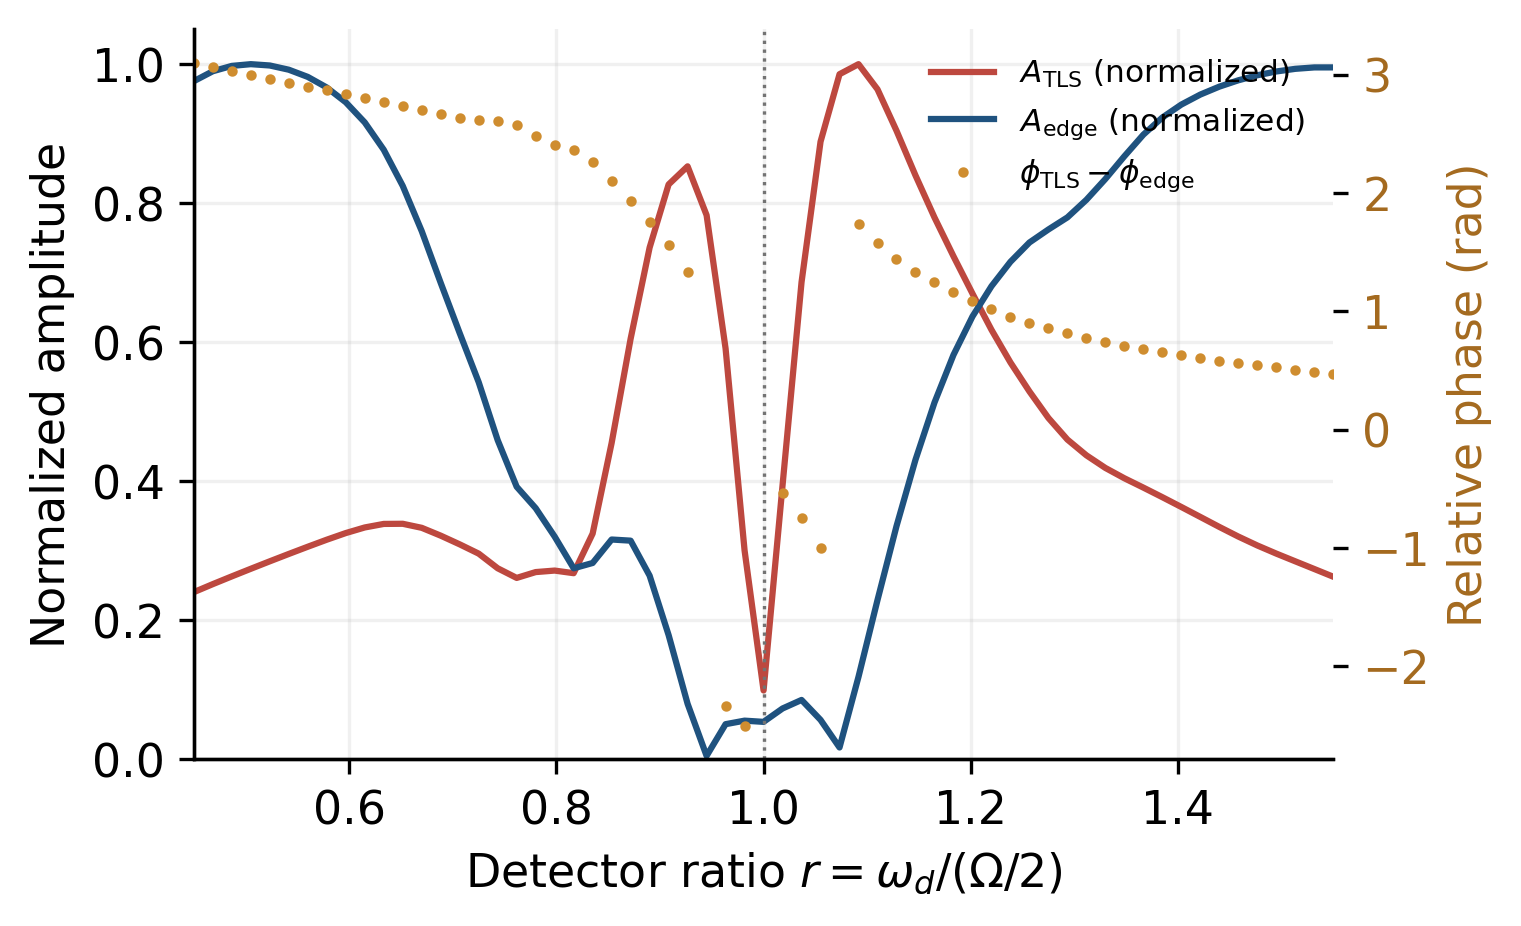
\includegraphics[width=0.78\textwidth]{figS5_detuning_phase.png}
\caption{Normalized TLS and edge amplitudes versus detector ratio, with the visibility-masked relative phase. The amplitudes are normalized separately for display; the phase points are not a fitted susceptibility.}
\label{fig:supp-detuning-phase}
\end{figure}

\subsection{Closed-chain gap parity and local sideband convention}

\Cref{fig:supp-gap-sideband} records the precise closed-chain gap convention used to organize the BDI-labelled control points. From $\cos(\epsilon_kT)=\cos\alpha\cos\beta+\cos k\sin\alpha\sin\beta$, a zero gap closes at the even branches $\alpha-\beta=2n\pi$ or $\alpha+\beta=2n\pi$, while a $\pi/T$ gap closes at the corresponding odd branches. The displayed lines in the first quadrant are representatives, not the complete closure conditions. The remaining panels define the separate physical contact $x$ and sideband index $\ell$, and visualize the local matrix-element profile used only in the reduced-model interpretation.

\begin{figure}[ht]
\centering
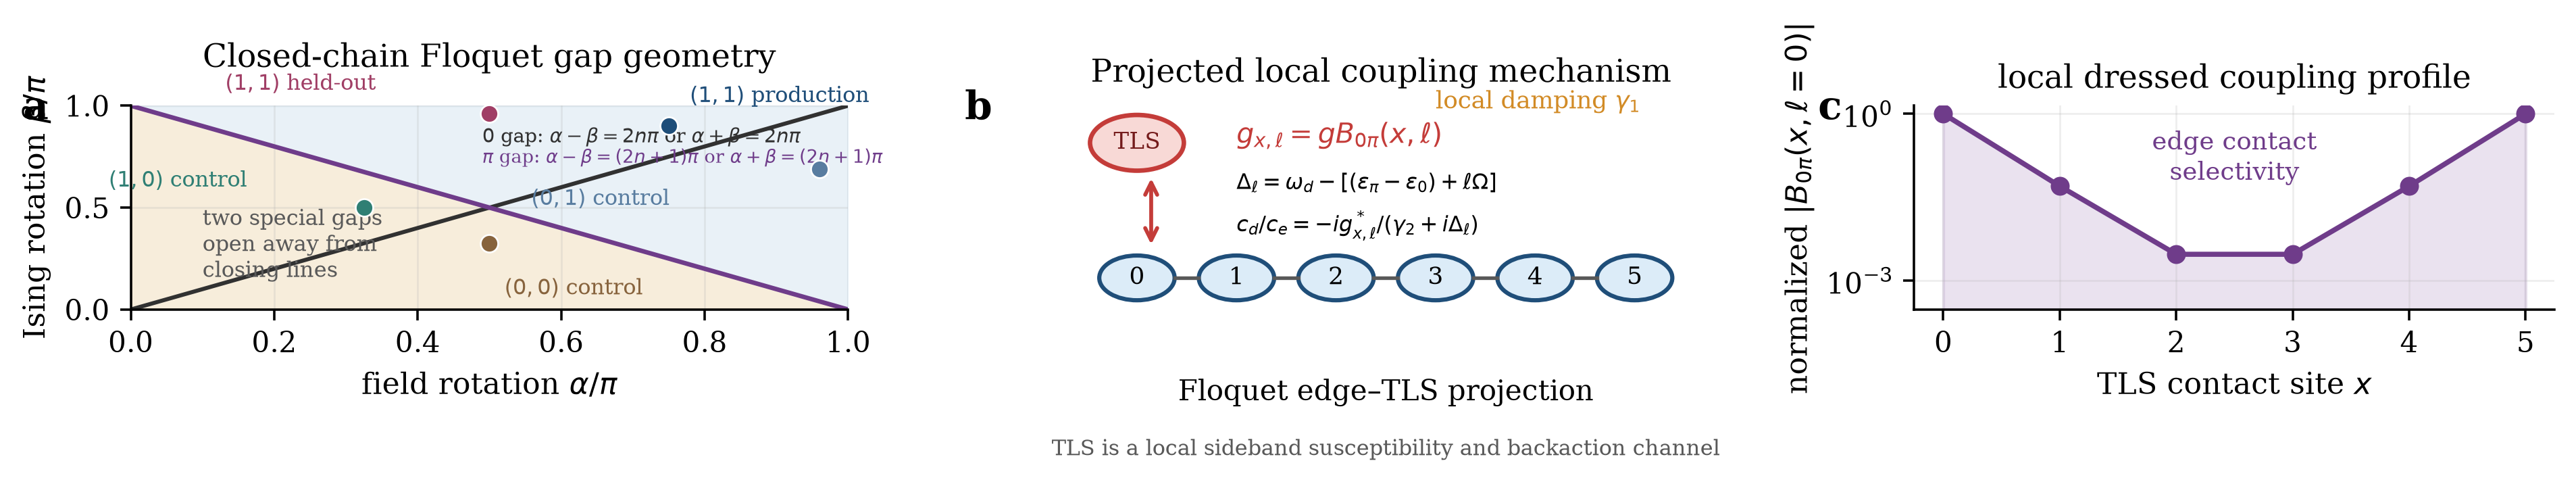
\includegraphics[width=\textwidth]{fig1_theory_edge_tls_coupling.png}
\caption{Supplementary closed-chain and projected-model convention. The BDI-labelled selected controls are checked against the correct even/odd gap-parity conditions. The $x$--$\ell$ sideband convention is interpretive; all principal curves remain full Floquet--Lindblad results.}
\label{fig:supp-gap-sideband}
\end{figure}

\subsection{Numerical construction of the BDI labels}

The closed-chain labels are computed before any TLS response is evaluated. For each candidate $(\alpha,\beta)$, the Bloch evolution is written in two symmetric time frames,
\begin{equation}
U_A(k)=U_1(k;\beta/2)U_2(\alpha)U_1(k;\beta/2),\qquad
U_B(k)=U_2(\alpha/2)U_1(k;\beta)U_2(\alpha/2).
\end{equation}
After the fixed basis rotation that exposes chiral off-diagonal form, the winding of the upper off-diagonal element $q_s(k)$ is evaluated on $4001$ uniformly spaced momenta over $[-\pi,\pi)$. Calling the resulting integers $w_A$ and $w_B$, the labels are
\begin{equation}
\nu_0=\frac{w_A+w_B}{2},\qquad \nu_\pi=\frac{w_A-w_B}{2}.
\end{equation}
A point is retained only when both off-diagonal functions remain nonzero on the sampled Brillouin zone, the two combinations above are integer-valued to numerical tolerance, and the quasienergy gaps are open. The stored margin is $\min_k\{\phi_k,|\pi-\phi_k|\}$, where $\phi_k=\arccos[\operatorname{Re}\operatorname{tr}U(k)/2]$. These labels select control drives only; they neither choose the dissipative initial state nor enter the full-model propagation.

\subsection{Prepared-pair and targeted-channel diagnostics}

The committed coupling scan provides the resolved-doublet phenomenology shown in the main text and the complete spectra in \cref{fig:supp-coupling-spectra}. The fit is restricted to branches resolved across the declared windows; it is not a global coupling law or an independent multi-position collapse. The prepared-pair/channel figure below is a separate mechanism diagnostic. Its exact N=4 component is useful for checking a channel/time bridge, but it must not be read as a complete N=6 channel spectrum.

\begin{figure}[ht]
\centering
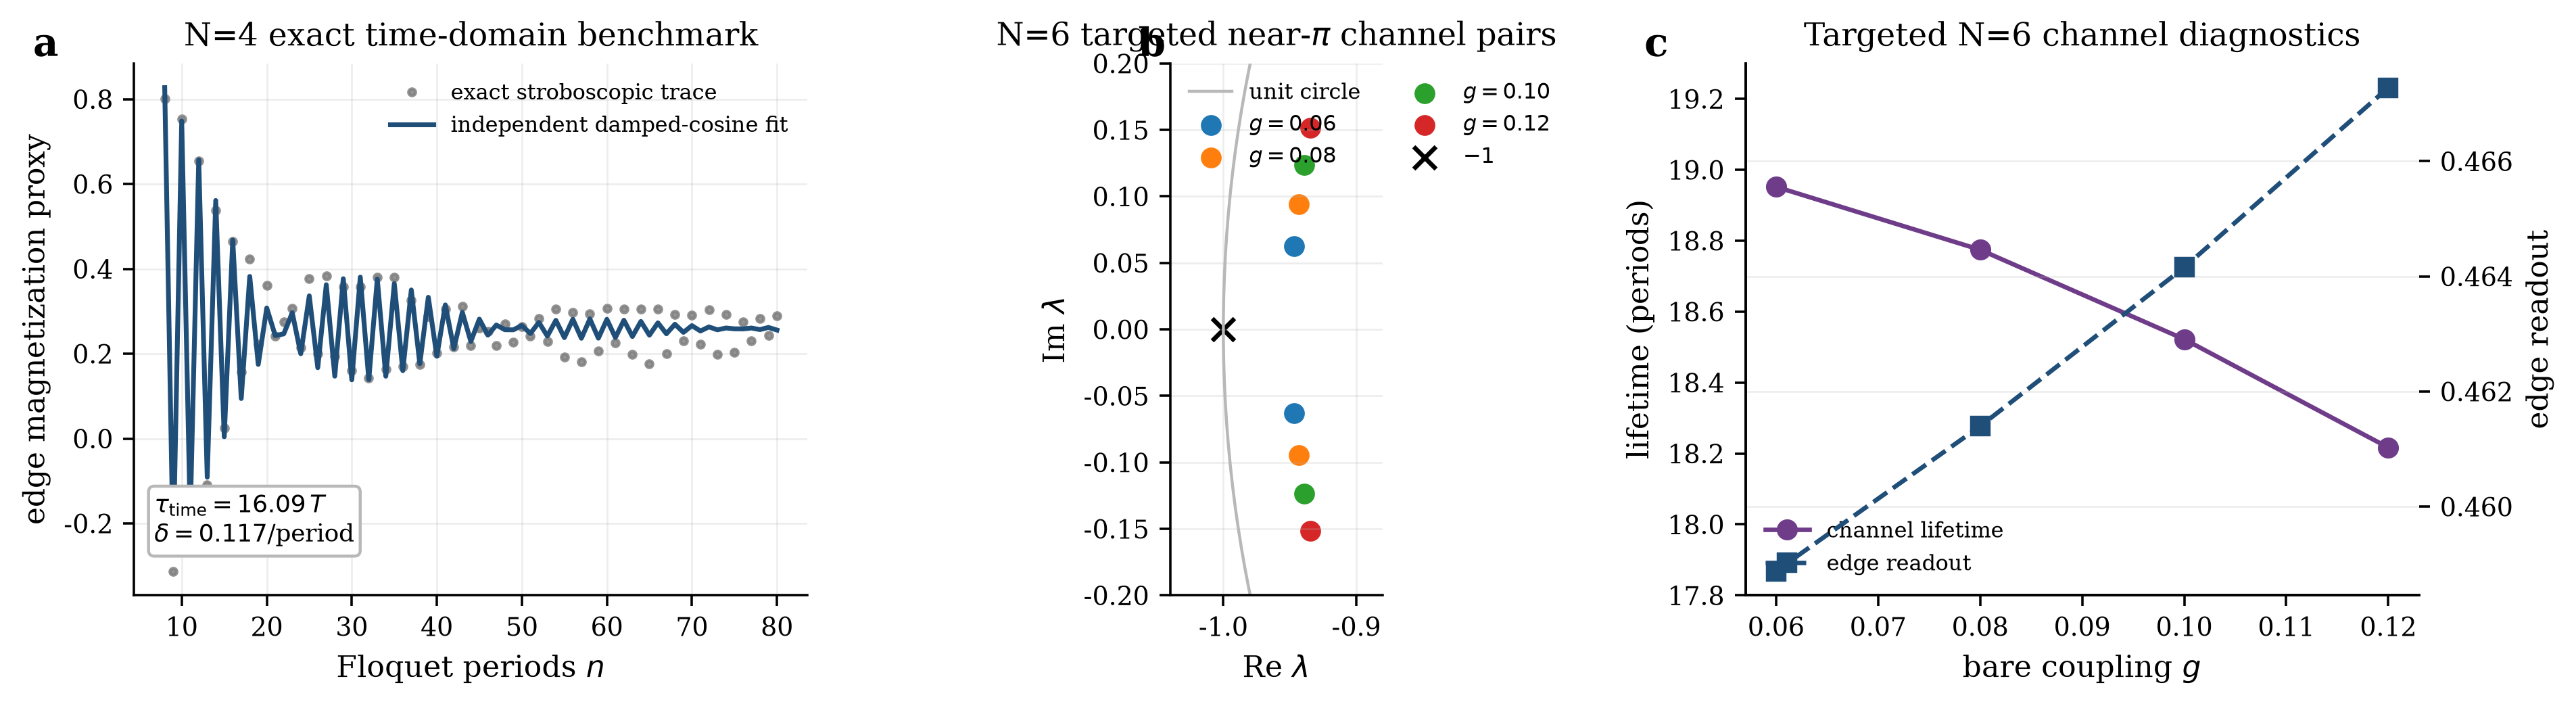
\includegraphics[width=\textwidth]{fig3_nearpi_channel_dynamics.png}
\caption{Supplementary near-$\pi$ channel/time diagnostic. The exact N=4 channel calculation is compared to an independent time-domain analysis; targeted N=6 records are residual-qualified near-$-1$ Ritz evidence with nonzero edge visibility, not an exhaustive channel/time validation.}
\label{fig:supp-nearpi}
\end{figure}

\subsection{Legacy formal multichannel truncation audit}

The formal $K$-channel controls use a Floquet-pair-prepared projected state and therefore have a different preparation contract from Gate A v3. They compare the normalized TLS response of the projected calculation, $a_K$, with the matched full response, $a_{\rm full}$, through
\begin{equation}
\epsilon_{\rm spec}(K)=\left\|\frac{a_{\rm full}}{\|a_{\rm full}\|_2}-\frac{a_K}{\|a_K\|_2}\right\|_2.
\end{equation}
The committed audit values are listed in \cref{tab:supp-k-audit}. At $g=0.08$, the dominant improvement occurs from $K=2$ to $K=4$ for both $N=6$ and $N=8$, while further channels change the error only modestly. The $N=8$, $g=0.12$ control remains nonpredictive throughout the tested $K=4$--$8$ range. These records delimit one tested reduced representation; they neither validate the common-product response nor prove that every alternative larger subspace must fail.

\begin{table}[ht]
\centering
\caption{Committed normalized spectral-error audit for the legacy formal $K$-channel controls.}
\label{tab:supp-k-audit}
\begin{tabular}{lrrrr}
\toprule
Control & $K=2$ & $K=4$ & $K=6$ & $K=8$ \\
\midrule
$N=6$, $g=0.08$ & 0.3646 & 0.1467 & 0.1442 & 0.1610 \\
$N=8$, $g=0.08$ & 0.3466 & 0.1452 & 0.1413 & 0.1384 \\
$N=8$, $g=0.12$ & 0.2950 & 0.6287 & 0.6220 & 0.6133 \\
\bottomrule
\end{tabular}
\end{table}

\subsection{Reduced-model failure at interior contacts}

The legacy Gate B2/C1 high-bare-coupling continuation toward interior contacts was performed precisely to test whether a single local dressed scale could collapse the spectra beyond the edge regime. It did not: peak rearrangement, detuning shifts, and window sensitivity prevent a universal multi-position line. This negative result is retained because it limits the otherwise useful edge-contact susceptibility language.

\begin{figure}[ht]
\centering
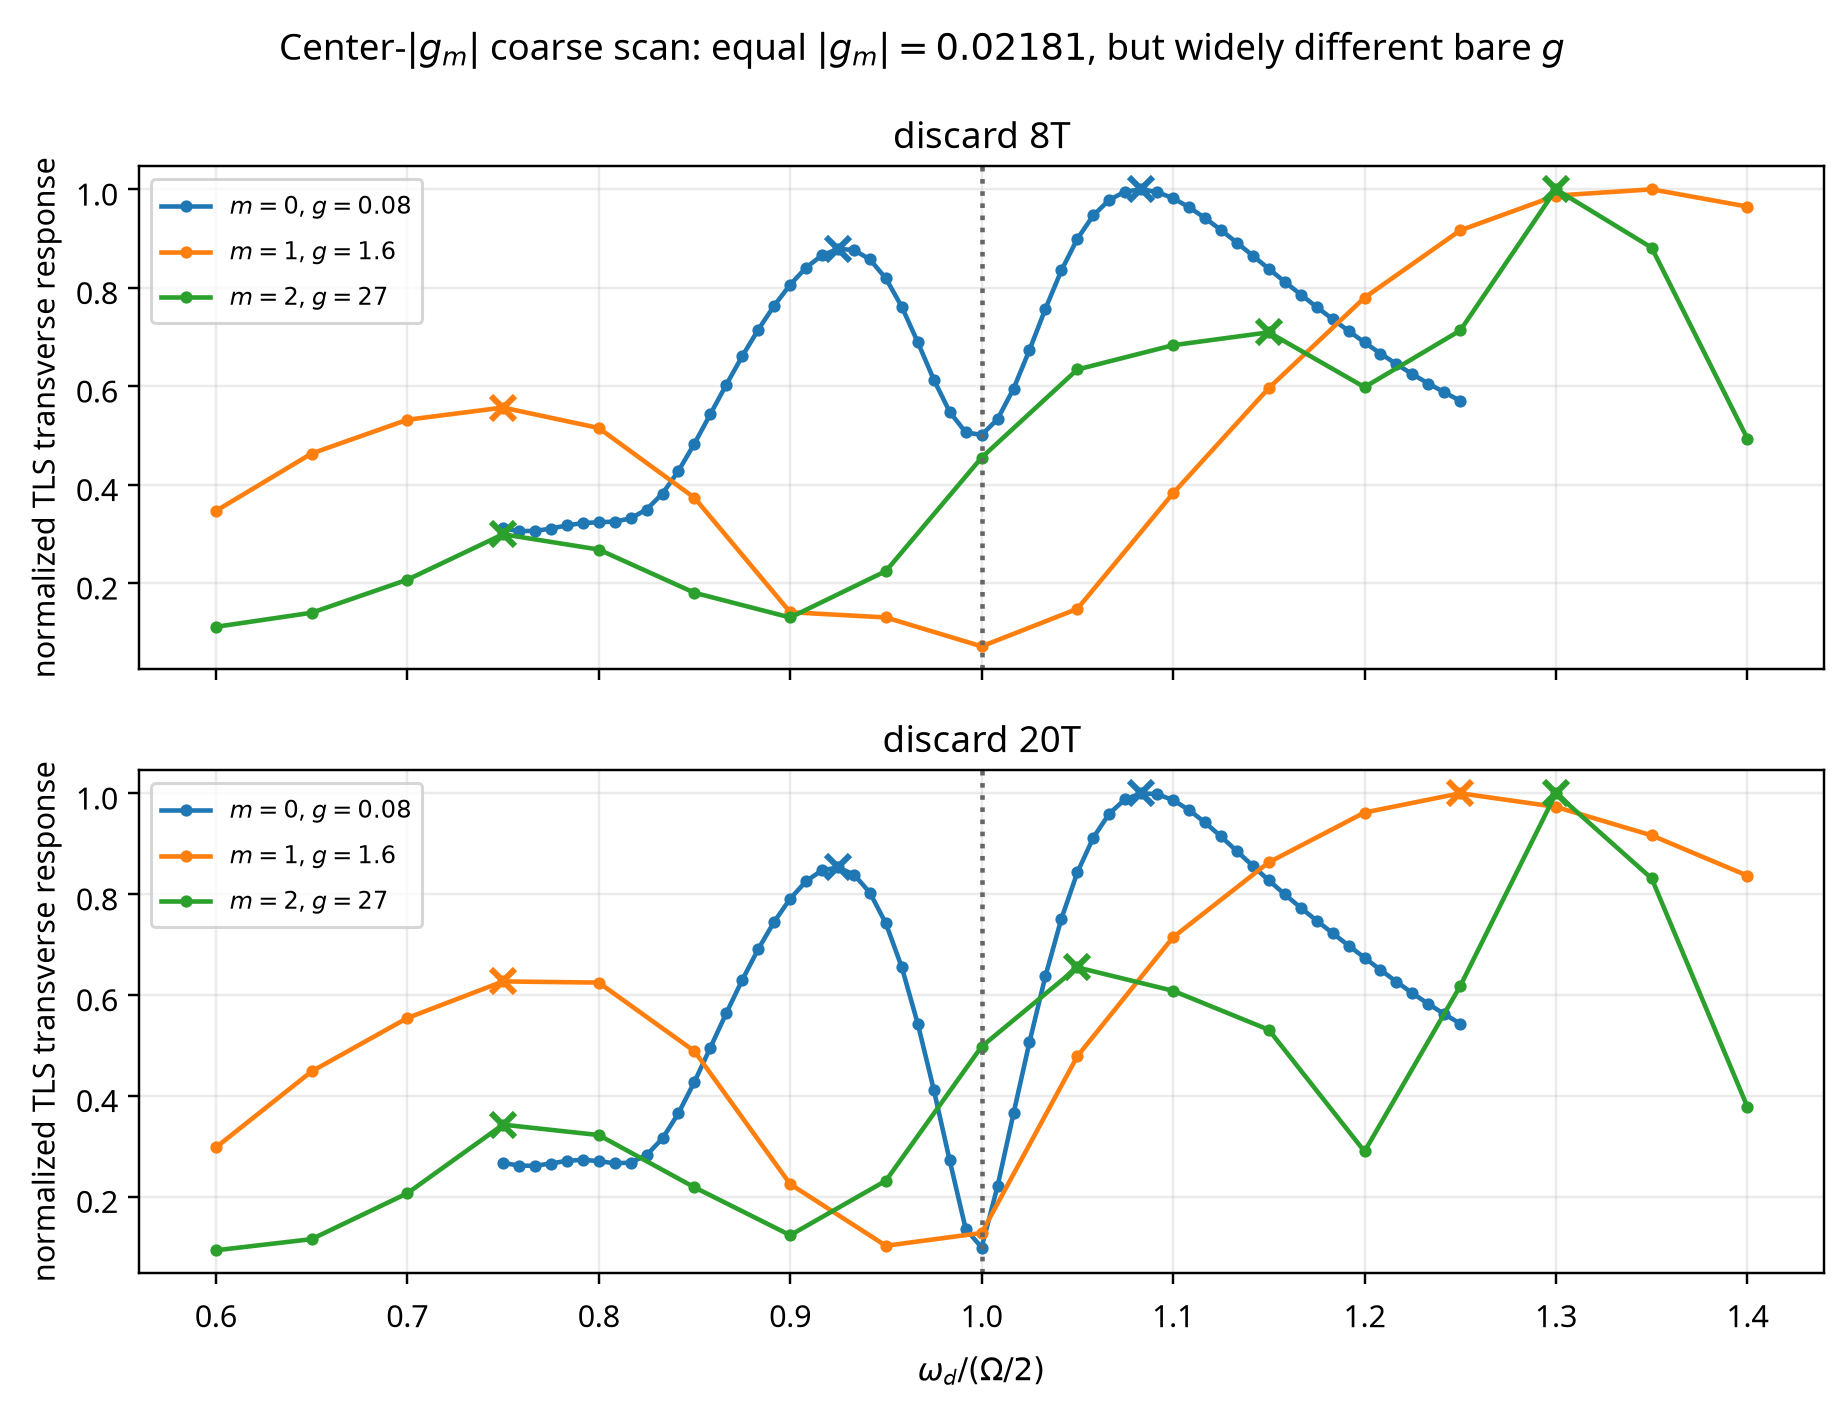
\includegraphics[width=0.82\textwidth]{figS4_reduced_model_failure.png}
\caption{Supplementary Gate B2/C1 reduced-model failure record for the coarse interior continuation. The spectra do not support a universal multi-position effective-coupling collapse at the required large bare couplings.}
\label{fig:supp-reduced-failure}
\end{figure}

\clearpage
\section{Exact channel/time benchmark and targeted channel records}
\label{sec:supp-channel}

The exact benchmark is prepared at $N=4$, $g=\gamma_1=0.08$, $\omega_d=\Omega/2$, and $T=2.591813939212$. Exact diagonalization of the one-period channel selects the conjugate pair
\begin{equation}
\lambda_\pm=-0.939373778674\mp\ii\,0.097672201737,
\end{equation}
The pair has modulus $0.944437904286$ and lifetime $17.4931177$ periods. Its absolute phase offset is $0.1036036$ rad per period. Each mode has edge-readout visibility $0.2110623$; the conjugacy residual is $9.94\times10^{-15}$.

An independent stroboscopic time-domain fit starts at period $n=8$. It gives $\tau_{\rm fit}/T=16.0915858$, $|\delta_{\rm fit}|=0.1167385$ rad per period, and RMSE $0.0299413$. It is not initialized with channel spectral information. The sensitivity to the discarded transient is listed in \cref{tab:supp-window}; it motivates the main-text language of quantitative compatibility rather than exact one-pole dynamics.

\begin{table}[ht]
\centering
\caption{Window sensitivity of the independent N=4 time-domain fit.}
\label{tab:supp-window}
\begin{tabular}{rrrr}
\toprule
Fit start $n$ & $\tau_{\rm fit}/T$ & $|\delta_{\rm fit}|$ (rad/period) & RMSE \\
\midrule
0 & 14.9577 & 0.106487 & 0.04662 \\
4 & 15.4084 & 0.113656 & 0.03768 \\
8 (primary) & 16.0916 & 0.116739 & 0.02994 \\
12 & 17.6021 & 0.118565 & 0.02943 \\
16 & 23.8719 & 0.118748 & 0.02833 \\
\bottomrule
\end{tabular}
\end{table}

At N=6, the reported records are residual-qualified, edge-seeded conjugate Ritz pairs near $-1$ with nonzero edge visibility for $g=0.06$--$0.12$. They are targeted near-$-1$ Ritz evidence, not an exhaustive N=6 Floquet-channel spectrum and not an N=6 channel/time lifetime-equality test. The full targeted records, residuals, and Krylov histories are available in the repository artifacts.

\section{Gate A v3 common-preparation and geometry controls}
\label{sec:supp-gatea}

Every principal Gate A v3 trajectory starts from the same physical state,
\begin{equation}
\rho(0)=\left(\ket{\uparrow_z}\bra{\uparrow_z}\right)^{\otimes N}\otimes\ket{0_d}\bra{0_d},\qquad N=6.
\end{equation}
Closed-chain labels $(\nu_0,\nu_\pi)$ index candidate controls only; they never select a Floquet-pair initial state, numerical mode index, or topology-dependent phase convention in the dissipative propagation. The fixed detector grid is
\begin{equation}
r=\omega_d/(\Omega/2)\in\{0.880,0.904,0.928,0.952,0.976,1.000,1.024,1.048,1.072,1.096,1.120\}.
\end{equation}

\begin{table}[ht]
\centering
\begin{threeparttable}
\caption{Gate A v3 controls and their logical role in the theory-driven paper.}
\begin{tabular}{>{\raggedright\arraybackslash}p{0.26\linewidth}>{\raggedright\arraybackslash}p{0.31\linewidth}>{\raggedright\arraybackslash}p{0.33\linewidth}}
\toprule
Control & Frozen setting & Interpretation boundary \\
\midrule
Production spatial profile & OBC $(1,1)$ drive; movable $x=0,\ldots,5$ & Six-contact boundary-selective readout, not an asymptotic length extraction. \\
Matched pair I & $(1,1)$ versus $(0,1)$; $T=2.591813939212$; $g=\gamma_1=0.08$ & Same-period directional comparison for this pair only. \\
Matched pair II & $(1,0)$ versus $(0,0)$; $T=1.295906969606$; $g=\gamma_1=0.16$ & Second pair; not a four-class common-period experiment. \\
Held-out geometry & $(1,1)$ OBC/PBC; $(\alpha/\pi,\beta/\pi)=(0.50,0.96)$ & Finite boundary-condition contrast, not a dissipative invariant. \\
Sampling/window & 2, 4, 8 samples; discards $8T$, $20T$, $40T$ & Deterministic numerical sensitivity, not statistical uncertainty. \\
\bottomrule
\end{tabular}
\end{threeparttable}
\end{table}

The production weights are $\Wraw(0)=3.3246564\times10^{-3}$, $\Wraw(1)=6.3758865\times10^{-4}$, and $\Wraw(3)=3.3874794\times10^{-6}$, giving $\Wraw(0)/\Wraw(1)=5.214$ and $\Wraw(0)/\Wraw(3)=981.45$. The held-out values are $W_{\rm r}^{\rm OBC}=2.5260841\times10^{-3}$ and $W_{\rm r}^{\rm PBC}=2.6485984\times10^{-7}$, giving the declared contrast $9537.44$. The audit forms these ratios from the finite stored values and applies no denominator floor or clipping. Relative to the baseline, normalized-shape distances for the two sampling variants are $0.00106$ and $0.000311$; the intentionally early and late discards yield $0.176876$ and $0.046216$. These checks support the stated finite response analysis but do not transform it into a thermodynamic boundary diagnostic.

\clearpage
\section{Response-blind Gate D1/D2 finite-size transfer}
\label{sec:supp-gated}

Gate D2 tests one frozen proposition: whether a stratified raw integrated-weight hierarchy selected at $N=4$ survives at $N=6$ for precisely the same eight drives and detector grids. The corrected D1 audit SHA-256 is
\begin{center}
\texttt{34961d819b8dd4cf1f1aaec519161e3d0a2674a5a043e660ad05d00770357f3a},
\end{center}
and the frozen D2 protocol SHA-256 is
\begin{center}
\texttt{e615217fa6063ff9c2d400cb927f9d1963d4a29386047fa3c6ae1c40335cd72e}.
\end{center}
Before accepting any task, the runner checks source-freeze commit, D1 anchors, field-by-field task identity, environment provenance, runner/helper hashes, ratio-grid identity, and resume integrity. The completed read-only audit independently rechecks result and self-hashes, schema, normalized shapes, and recomputed $\Wraw$.

\begin{table}[ht]
\centering
\caption{Frozen Gate D2 decision components.}
\begin{tabular}{lll}
\toprule
Component & Threshold & Completed value \\
\midrule
Median ratio at fixed $\nu_0=0$ & $>10$ & $409.535710509421$ \\
Median ratio at fixed $\nu_0=1$ & $>10$ & $5633.719777194818$ \\
Strict ordering $\min W_{\nu_\pi=1}/\max W_{\nu_\pi=0}$ & $>1$ & $12.048022303011$ \\
\bottomrule
\end{tabular}
\end{table}

\begin{table}[ht]
\centering
\caption{All eight task-level raw weights used in the finite-size transfer figure. Drive IDs are the exact frozen task identifiers; no interpolation or point replacement is performed.}
\label{tab:supp-d2-points}
\small
\begin{tabular}{lrrr}
\toprule
Drive ID & Period $T$ & $W_{\rm r}(N=4)$ & $W_{\rm r}(N=6)$ \\
\midrule
\texttt{nu00\_a} & 1.212655 & $2.797244\times10^{-4}$ & $1.632143\times10^{-4}$ \\
\texttt{nu00\_b} & 1.212655 & $3.686111\times10^{-7}$ & $3.109834\times10^{-7}$ \\
\texttt{nu10\_a} & 1.212655 & $1.175303\times10^{-6}$ & $8.937595\times10^{-7}$ \\
\texttt{nu10\_b} & 1.212655 & $1.065398\times10^{-7}$ & $7.593314\times10^{-8}$ \\
\texttt{nu01\_a} & 2.318495 & $3.575519\times10^{-2}$ & $3.575451\times10^{-2}$ \\
\texttt{nu01\_b} & 2.617994 & $3.121586\times10^{-2}$ & $3.121494\times10^{-2}$ \\
\texttt{nu11\_a} & 2.318495 & $1.959268\times10^{-3}$ & $1.966410\times10^{-3}$ \\
\texttt{nu11\_b} & 2.617994 & $3.522754\times10^{-3}$ & $3.496567\times10^{-3}$ \\
\bottomrule
\end{tabular}
\end{table}

All three frozen conditions pass. The result establishes a finite, response-blind, cross-period persistence statement for this eight-drive hierarchy. It does not establish a common-period causal $\nu_\pi$ law, a universal TLS line shape, a thermodynamic invariant, or a phase boundary.

\section{Reproduction commands and artifact policy}
\label{sec:supp-reproduction}

The repository checks the committed evidence without repeating the production propagation:
\begin{verbatim}
python scripts/run_submission_checks.py --check-only
\end{verbatim}
This check includes the independent Gate A v3 and D2 audits and figure-record checks. Individual commands for regenerating figures from committed records are documented in the \href{https://github.com/666888rwy-bit/floquet-tls-pi-edge-tls}{public repository}'s \texttt{manuscript/README.md}. The frozen protocols, raw-result manifests, and hashes are retained in the D2 result commit \texttt{a3d9dc3}. A version-specific archival DOI for the present manuscript has not yet been assigned.

\end{document}
